\documentclass{report}

\usepackage[utf8]{inputenc}
\usepackage[T1]{fontenc}
\usepackage[french]{babel}

\usepackage{lmodern}

\usepackage{setspace}
\spacing{1.5}

\usepackage[top=2.5cm, bottom=2.5cm, left=2.5cm, right=2.5cm]{geometry}

\usepackage{url}

\usepackage{graphicx}

\usepackage{array,multirow,makecell,tabularx}
\renewcommand\tabularxcolumn[1]{>{\centering\arraybackslash}m{#1}}
\usepackage{booktabs}
\usepackage{floatrow}
% Table float box with bottom caption, box width adjusted to content
\newfloatcommand{capbtabbox}{table}[][\FBwidth]

\usepackage{pdfpages}

\usepackage{listings}
\usepackage{minted}

\usepackage{hyperref}

\usepackage{titlesec} 
\titleclass{\part}{top} % changing part so that it does not take a full page.
\titleformat{\part}
    [display] % shape
    {\centering\normalfont\Huge\bfseries} % format
    {\MakeUppercase{\partname}\vspace{1pc}} % label
    {0pt} % set between label and title body
    {\titlerule[2pt]\vspace{1pc}\Huge\MakeUppercase} % before body
\titlespacing*{\part}
    {0pt} % left 
    {0pt} % before sep
    {10pt} % after sep

\titleclass{\chapter}{straight} % make chapter like a section (no newpage)
\titleformat{\chapter}
    [display] % shape
    {\centering\normalfont\huge\bfseries} % format
    {\chaptertitlename ~\thechapter} % label 
    {0pt} % sep between label and title body
    {\huge\MakeUppercase} % before body
\titlespacing*{\chapter}
    {0pt} % left
    {20pt} % before sep
    {20pt} % after sep

\usepackage{chngcntr}
\counterwithout{figure}{chapter}
\counterwithout{table}{chapter}
    

\newcommand{\emphbox}[1]{
    \vspace{5mm}
    \noindent\fbox{ 
        \begin{minipage}[c]{\linewidth}
            {\em #1}
        \end{minipage}
    }
}

\newcommand{\reffig}[1]{F\textsc{igure}~\ref{#1} page~\pageref{#1}}

\newcommand{\reftable}[1]{T\textsc{able}~\ref{#1} page~\pageref{#1}}

\newcommand{\mref}[1]{\ref{#1} page~\pageref{#1}}

\title{Extraction de données relatives aux produits alimentaires à partir de documents non structurés}
\author{Pierre \textsc{massé}}
\date{Juin 2020}

\begin{document}

\maketitle

\large
\begin{abstract}
    {\em
    
    La gestion de l'information produit est devenu un enjeu de société majeur ces dernières années.
    Les scandales sanitaires récents ont déclenché une prise de conscience collective des consommateurs, en parallèle de la mise en place de réglementations de plus en plus contraignantes pour l'ensemble des acteurs de la filière~\cite{incotext}\cite{incoexpl}.
    \`{A} ce titre, le Groupe Pomona a lancé ces dernières années un projet majeur de refonte des processus et des outils de gestion de l'information produit.

    La première filiale du Groupe a fait l'objet d'un déploiement réussi, mais cela a toutefois mis en évidence le fait que des gains à la fois en qualité et en productivité restent accessibles.

    La mise en place d'outils mettant en oeuvre les principes du Machine Learning appliqués au traitement du langage permettrait d'aider les opérationnels de la gestion de l'information à interpréter plus vite et mieux les documents mis à disposition par les fournisseurs du Groupe.

    Le présent rapport détaille la mise en place d'un outil permettant d'extraire les listes d'ingrédients des fiches techniques transmises par les fabricants des produits.
    }
\end{abstract}
\normalsize

\tableofcontents

\part{Contexte métier}

    \chapter{Description du Groupe}

    \large
    L'objet de l'ensemble de cette première partie est de donner sur le Groupe Pomona des éclairages nécessaires à la compréhension du cas d'usage développé.
    Bien d'autres aspects sur la société, pourraient être mentionnés (ex : des indicateurs sur l'activité, l'histoire du Groupe\dots) mais ils seront omis car non indispensables à la compréhension du sujet.
    Plus de détails sur le Groupe sont accessibles sur le site web de la société\cite{site_pomona}.
    \normalsize    

        \section{Le métier du Groupe Pomona}
        \label{business}

        Le Groupe Pomona est une société de distribution livrée de produits alimentaires à destination des professionnels des métiers de bouche.
        L'activité du Groupe consiste uniquement à acheter et revendre de la marchandise, à l'exclusion de toute activité de fabrication ou de transformation\footnote{de très rares cas de transformation existent (ex : mûrissage de fruits, filetage de poisson) mais sont extrêmement exceptionnels}. Le Groupe Pomona est une société de \emph{distribution}. Elle ne possède d'ailleurs pas d'actif industriels (autre que des entrepôts logistiques) ni d'agréement pour transformer les marchandises.        
        
        Cette activité d'achat/vente se fait dans la majorité des cas sous le régime du \emph{négoce}, à savoir que le Groupe acquiert la propriété des marchandises qu'il commercialise avant de la céder à ses clients.
        L'autre régime est celui dit de la \emph{prestation (logistique)}.
        Dans ce cas, par le jeux d'écritures comptables, la valorisation du stock disparaît des comptes du Groupe.
        Néanmoins, indépendamment de cet aspect purement comptable, l'ensemble :
        \begin{description}
            \item[des flux de documents :] commandes d'achat, factures fournisseur, commandes de vente, factures clients
            \item[des flux financiers :] paiements fournisseur, paiements client
            \item[des flux physiques :] réception et stockage, préparation et expédition
        \end{description}
        restent largement inchangés.
        
        Pour résumer, l'activité de l'ensemble des entités du Groupe pourraient se résumer via le schéma présenté à la \reffig{fig:flux metier}

        \begin{figure}[htbp]
            \begin{center}
            \includegraphics[width=\linewidth]{img/Les flux métier de Pomona.png}
            \end{center}
            \caption{Les flux métier avec les partenaires commerciaux}
            \label{fig:flux metier}
        \end{figure}

        \emphbox{Le métier du Groupe est d'être un \emph{grossiste}, qui achète et revend des produits alimentaires\footnotemark \ \emph{sans produire ou transformer quoi que ce soit}.}
        \footnotetext{dans la grande majorité des cas, cf. \emph{Les produits non-alimentaires} \mref{produits_nonal}}

        \section{La décentralisation}
        
        Le Groupe Pomona est un Groupe fortement décentralisé, avec des organisations largement indépendantes les unes des autres. 

            \subsection{Les Directions fonctionnelles}

            Pour des raisons évidentes de recherche de synergies ou de conformité réglementaires, certaines activités restent toutefois mutualisées à la maille du Groupe.
            Il s'agit des organisations suivantes :
            \begin{description}
                \item[La Direction Administrative et Financière (DAF) :] regroupe les équipes comptables Groupe, l'audit interne et la consolidation financière
                \item[La Direction Qualité :] est en charge de définir et contrôler l'application des standard de qualité
                \item[La Direction des Systèmes d'Information (DSI) :] développe et maintient en condition opérationnelles les systèmes d'information du Groupe
                \item[La Direction Technique et Logistique (DTL) :] est en charge des projets immobiliers (entrepôts), des négociations avec les transporteurs et joue un rôle de conseil interne sur les sujets logistiques
                \item[La Direction des Ressources Humaines :] se charge de l'ensemble des aspects en lien avec le recrutement, la paye et les sujets sociaux
                \item[La Direction Commerciale Groupe (DCG) :] définit une stratégie et des bonnes pratiques commerciales et marketing
            \end{description}

            \subsection{Les clients du Groupe}
            \label{clients}

            Afin de comprendre l'organisation du Groupe, il est nécessaire de connaître la typologie de ses clients.
            Comme mentionné précédemment, le Groupe s'adresse exclusivement aux professionnels des métiers de bouche.
            Aucune marchandise n'est vendue à des particuliers.
            Les principales typologies de clients sont les suivantes : 
            \begin{description}
                \item[Les Sociétés de Restauration :] elles exploitent les restaurants d'entreprise et certaines cantines d'établissement d'enseignement supérieur
                \item[Les Marchés Publics :] regroupent les clients qui dépendent des collectivités (écoles, hôpitaux, prisons, \dots)
                \item[La restauration commerciale :] est l'ensemble des restaurants à vocation commerciale, qu'ils soient chaînés (hippopotamus, O'Tacos, \dots) ou indépendants (\og le restaurant du coin \fg)
                \item[Les spécialistes :] il s'agit des détaillants spécialisés qui s'adressent aux particuliers. Boulangers, pâtissiers, bouchers, traiteurs, vente à emporter, \dots
                \item[Les Grandes et Moyennes surfaces (la GMS) :] sont les enseignes de la grande distribution. En général, l'accès à ces clients est compliqué par les règles mises en place par leurs centrales d'achat. Il représentent en général qu'un canal de vente d'opportunité.
            \end{description}

            Les trois premières de ces catégories représentent ce que l'on appelle la \emph{Restauration Hors Domicile (RHD)} (ou parfois également la Restauration Hors Foyer, RHF).

            \subsection{Premier niveau de décentralisation : les branches}
            \label{les_branches}
            Le Groupe Pomona est divisé en branches, qui sont des organisations indépendantes et qui ont toute latitude pour gérer leurs stratégie et politique commerciales, la gestion de leurs achats, leur stratégie marketing, \dots
            En particulier, les systèmes d'information ne sont pas identiques entre les différentes branches.
            Afin d'éviter de se concurrencer entre elles, leurs domaines d'activité respectifs ont été partitionnés par familles de produit commercialisés, segments client cibles et géographie. 

                \subsubsection{Les branches RHD}
                
                Les branches RHD s'adressent comme leur nom l'indique aux client de la Restauration Hors Domicile (cf. section \mref{clients}) en France.
                Elles se répartissent ce marché en travaillant des gammes de produits distinctes.
                Il s'agit des branches historiques du Groupe, qui représentent l'essentiel de son chiffre d'affaire.
                La répartition par produit est la suivante :
                \begin{description}
                    \item[PassionFroid :] spécialiste des \emph{produits surgelés, de la viande fraîche et des produits laitiers}
                    \item[\'{E}piSaveurs :] spécialiste des produits qui se conservent à température ambiante : \emph{produits d'épicerie, conserves, boissons et consommables de cuisine non-alimentaires}
                    \item[TerreAzur :] spécialites des \emph{Fruits et Légumes frais, et Produits De la Mer frais} 
                \end{description}
                La non-concurrence entre les branches est assurée par le fait qu'elles ne commercialisent pas les mêmes produits.
                Bien que nommées RHD, elles peuvent également vendre leurs produits à la grande distribution, mais généralement ces marchés sont verrouillés par les centrales d'achat des grandes enseignes.
                De plus, les branches RHD utilisent le progiciel SAP comme système de gestion.
                La branche TerreAzur est en cours de déploiement, en 2020 environ les 2 tiers des succursales travaillent avec ce progiciel.

                \subsubsection{Les branches spécialistes}

                Les branches spécialistes s'adressent aux clients dits spécialistes (cf. section \mref{clients}) en France.
                Elles sont en mesure de commercialiser tout type de produit pour répondre aux besoins de leurs clients.
                En particulier, elles peuvent tout à fait commercialiser certains produits qui sont également vendus par les branches RHD.
                Elles se répartissent la clientèle spécialiste de la manière suivante :
                \begin{description}
                    \item[Délice et Création :] s'addresse aux \emph{Boulangers et Pâtissiers}
                    \item[Saveurs d'Antoine :] s'adresse aux \emph{Bouchers, Charcutiers et Traiteurs}
                    \item[Relais d'Or :] s'addresse à la \emph{restauration indépendante nomade}
                \end{description}
                Comme pour les branches RHD, ces branches peuvent lorsqu'elles en ont l'opportunité vendre leurs produits à la GMS.

                \subsubsection{L'étranger}

                Bien que le Groupe Pomona soit une société dont l'essentiel de l'activité est faite sur le marché français, deux réseaux sont en cours de constitution sur des pays limitrophe.
                Ces branches sont susceptibles de travailler tout type de produit, à destination de tout type de client.
                Elles sont positionnées sur les marchés suivants : 
                \begin{description}
                    \item[Pomona Suisse :] présente sur le marché Suisse
                    \item[Pomona Iberia :] présente sur le marché Espagnol 
                \end{description}

                On peut synthétiser la répartition de l'activité par branche de la manière présentée à la \reffig{fig:repartition_activite}.

                \subsubsection{Les produits non-alimentaires}
                \label{produits_nonal}
                Si l'essentiel des produits commercialisés par les branches du Groupe sont des produits alimentaires, comme évoqué précédemment une partie de l'activité commerciale se fait tout de même autour de produits non-alimentaires.
                Ces produits restent malgré tout destinés exclusivement aux professionnels des métier de bouche, et il s'agit de consommables (par opposition à des articles d'électroménager, de la vaisselle non-jetable, \dots).

                On distingue en général deux catégories de produits non-alimentaires : 
                \begin{itemize}
                    \item les produits dits \og d'hygiène \fg
                    \item les produits dits \og de chimie \fg
                \end{itemize}

                Les produits de chimie regroupent les produits qui doivent faire l'objet d'une fiche de données de sécurté au sens du réglement Européen No 1907/2006 dit \og REACH \fg (Registration, Evaluation, Authorisation and Restriction of Chemicals) \cite{reach_text}.

                Les produits d'hygiène regroupent tous les autres produits non-alimentaires.
                L'appelation \og d'hygiène \fg est donc réductricte, dans la mesure où cette large famille regroupe les consommables de nettoyage (éponges, papiers absorbants, \dots) mais également tout type d'autres consommables (serviettes de tables, gobelets en plastiques, pics à brochettes, boîtes de produits à emporter, \dots).

                \emphbox{La commercialisation de produits non-alimentaires existe au sein du Groupe, mais on se focalisera pour la suite sur les produits alimentaires qui reste le coeur de métier.}

                \begin{figure}[htpb]
                    \begin{center}
                    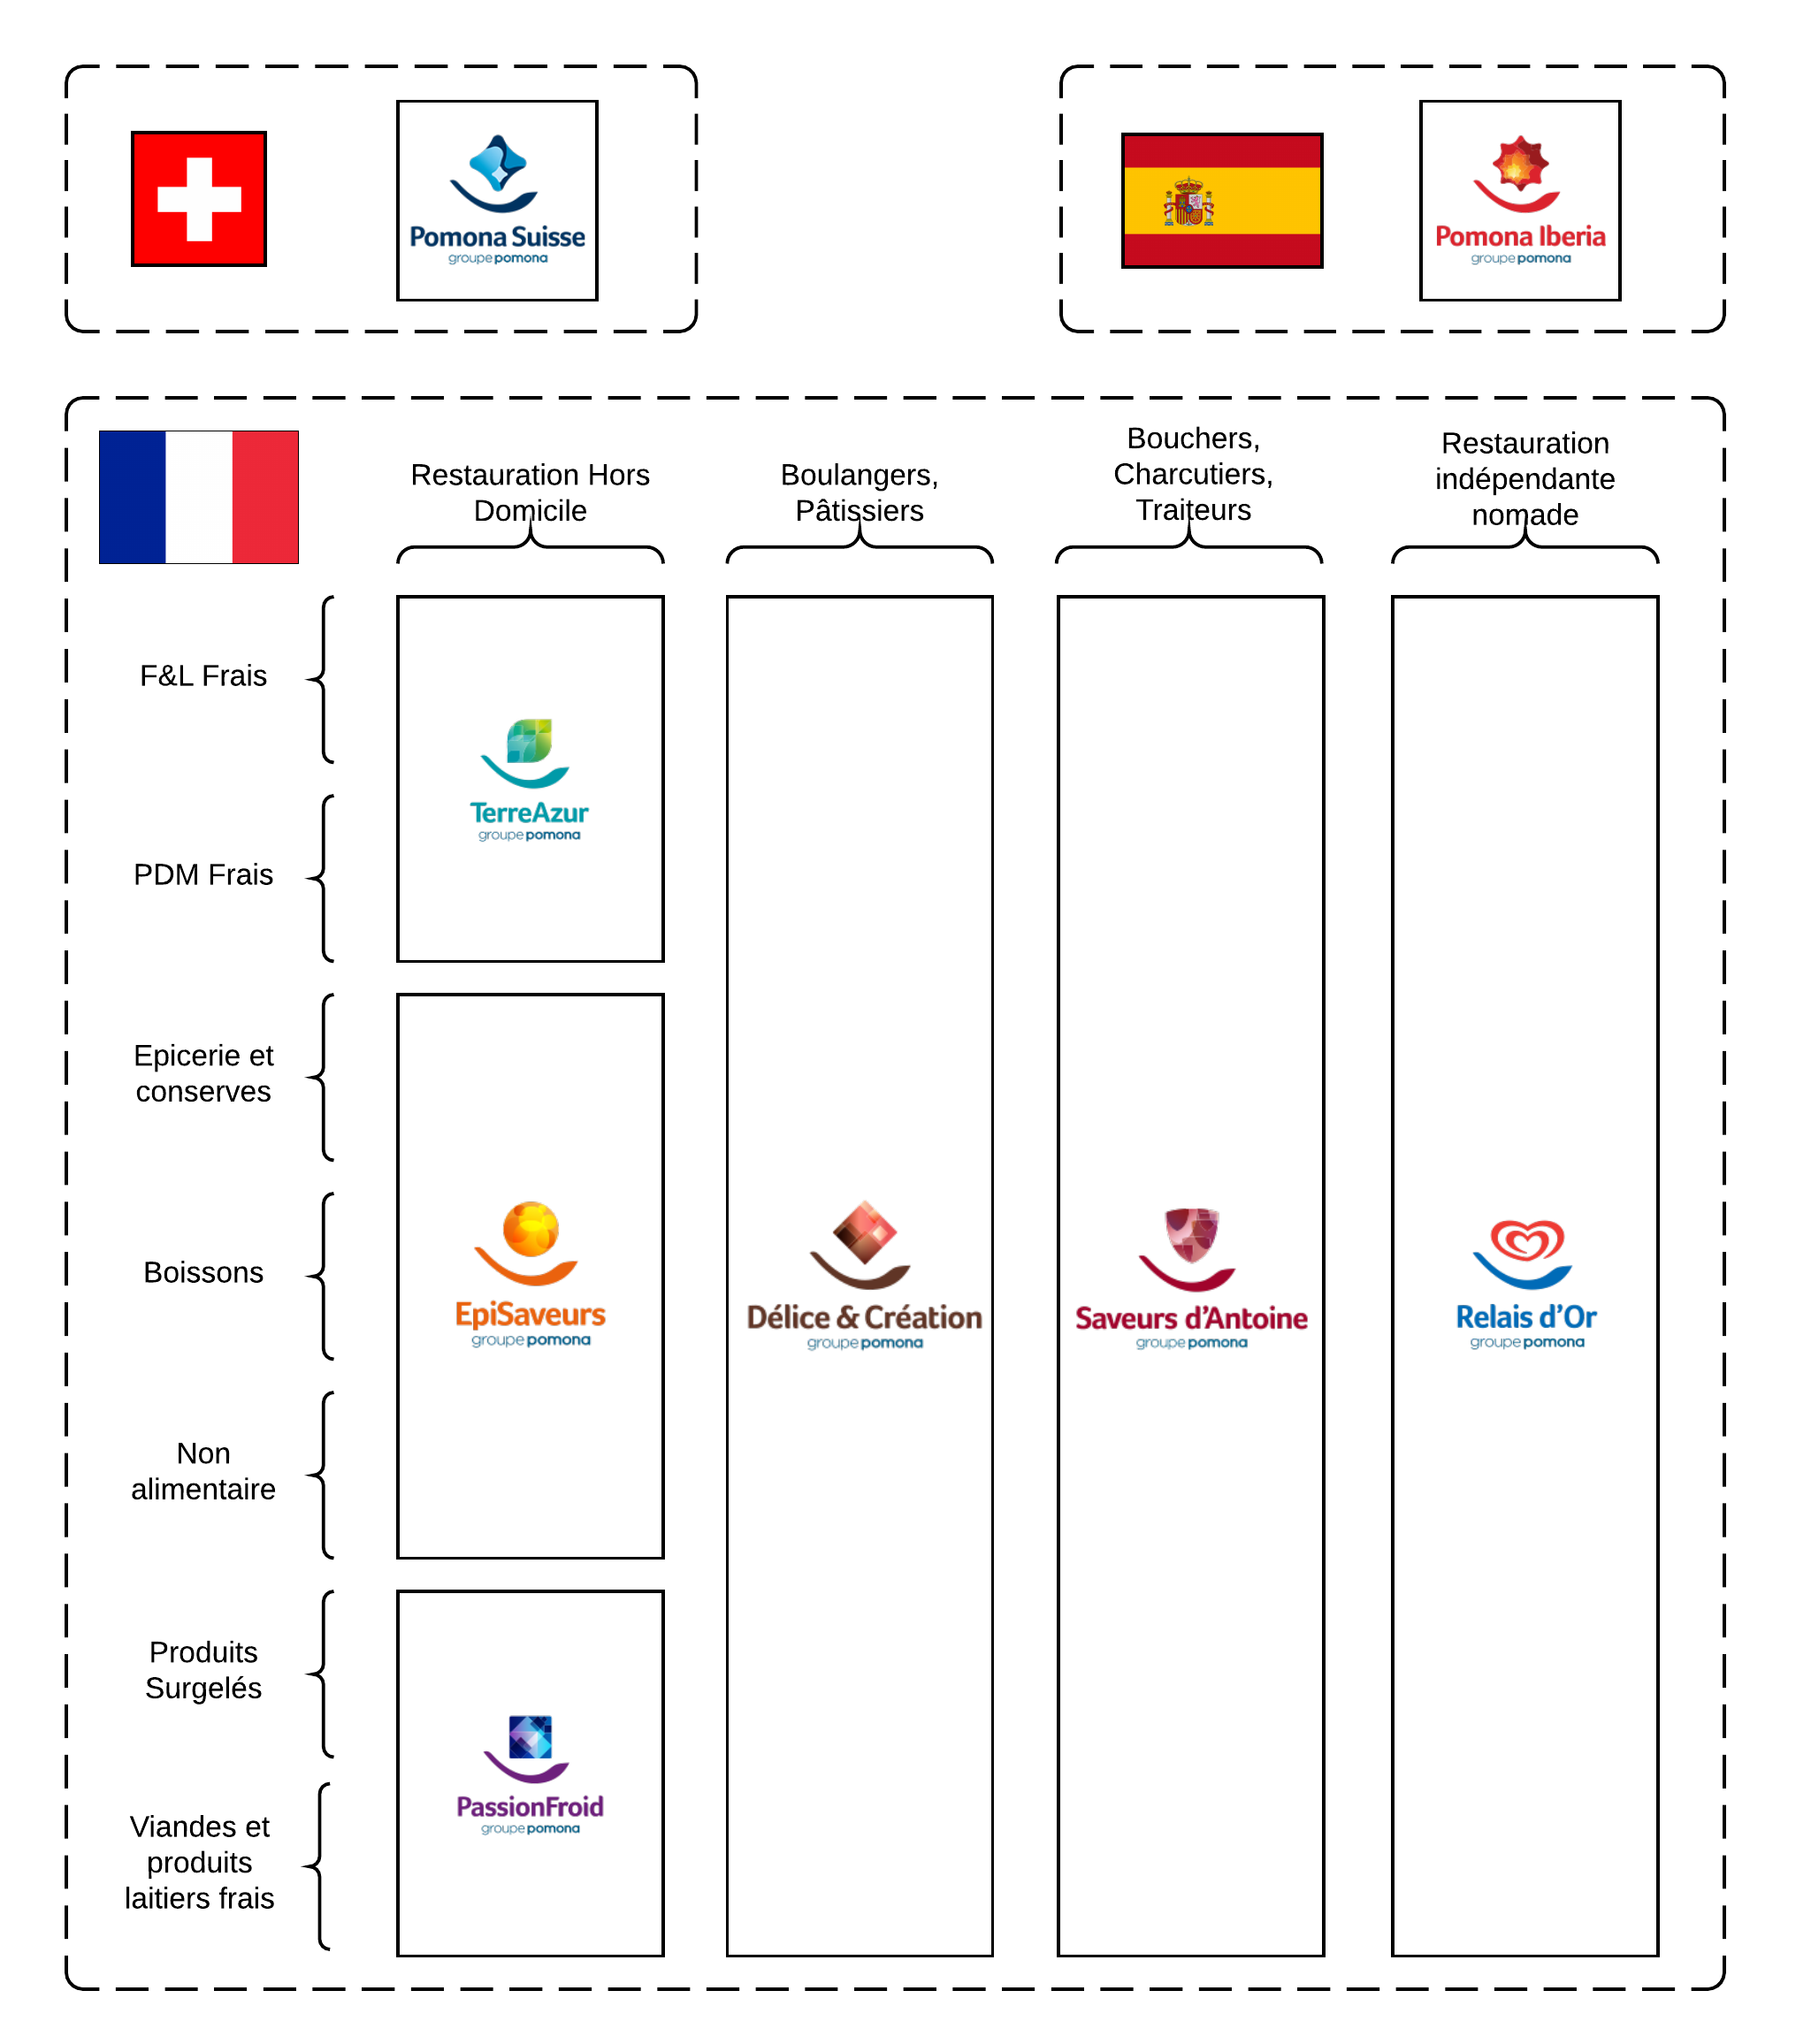
\includegraphics[width=\linewidth]{img/La répartition de l'activité des branches.png}
                    \end{center}
                    \caption{La répartition de l'activité des branches}
                    \label{fig:repartition_activite}
                \end{figure}

            \subsection{Le second niveau de décentralisation : les succursales}

            Chacune des branches est elle-même à son tour décentralisée en un réseau d'entrepôts régionaux : les succursales (parfois également appelées simplement \og régions\fg).
            Ces succursales sont gérées comme des PME indépendantes, avec un directeur et un compte de résultat qui leur est propre.
            Si certaines négociation avec des fournisseurs ou des clients nationaux sont parfois menée par les branches, les succursales sont autonomes dans :
            \begin{itemize}
                \item{la définition de leur assortiment, même si des contraintes s'appliquent}
                \item{la stratégie de développement commercial}
                \item{la négociation des prix d'achat}
                \item{la négociation des prix de vente}
                \item{la politique de rémunération de leurs employés}
            \end{itemize}
            
            \`{A} ce titre, elles ont leurs propres équipes d'achat, leurs équipes commerciales (télévente et vente route), leurs équipes administratives et évidemment leurs équipes logistiques (essentiellement en entrepôt et les chauffeurs livreurs en charge des livraisons client).

            Certaines activités restent de la responsabilité des équipes centrales des branches, comme : la négociation avec les clients ou les fournisseurs nationaux, la constitution de l'assortiment commun (les produits que toutes les succursales doivent détenir), la gestion des référentiels de données de base métier, \dots
            
            Un exemple de maillage régional est présenté en \reffig{fig:reseau_es}, sachant que ce maillage régional est différent pour chacune des branches.
            \begin{figure}[htpb]
                \begin{center}
                \includegraphics[width=\linewidth]{img/réseau es.png}
                \end{center}
                \caption{Le maillage régional de la branche \'{E}piSaveurs}
                \label{fig:reseau_es}
            \end{figure}


    \chapter{La gestion de l'information produit}
    
    \large
    Ce chapitre a pour vocation à éclairer les aspects métier en lien avec la gestion de l'information produit. 
    C'est le seul processus métier qui sera détaillé dans la mesure où c'est uniquement celui qu'il est nécessaire de connaître pour comprendre les cas d'usage développés ultérieurement.
    \normalsize

        \section{L'information produit}
        
            \subsection{Utilisations de l'information produit}
            \label{utilisation_info_produit}

                \subsubsection{Conformité réglementaire}
                La gestion de l'information produit est essentiellement une contrainte réglementaire à statisfaire.
                Comme mentionné au préambule, la réglementation autour de l'information des consommateur s'est sans cesse complétée au cours des dernières années.
                Un des textes centraux est le règlement n°1169/2011 dit INCO (INformation COnsommateur)\cite{incotext}\cite{incoexpl}.
                C'est ce règlement qui définit l'ensemble des informations qui doivent être étiquetées sur le produit (liste d'ingrédients, tableau de données nutritionnelles, \dots), mais également affichée au client lors de commande en ligne sur les sites de e-commerce.
                Il s'agit principalement d'informations relatives à la sécurité alimentaire (ex : les allergènes) ou la santé (ex : informations nutritionnelles).

                \subsubsection{Attentes client}

                Les consommateurs finaux (les \og convives \fg) étant de plus en plus sensibles au contenu de leur assiète, les clients du Groupe sont de plus en plus demandeurs d'information relatives aux produits qu'ils commandent.
                Ils demandent donc régulièrement des informations qui vont au-delà de ce qui est normalement prévu par la réglementaition.

                De plus, sur certains marchés pour lesquels des contrats courant sur de longues périodes - jusqu'à un an - sont établis (les marchés publics sont très concernés), il n'y a pas d'échantillonnage des produits.
                La seule manière pour ces clients d'évaluer la qualité des produits est de se référer aux documents contenant les informations produit, fournis par les distributeurs.

                \subsubsection{Gestion}

                Certaines informations relatives au produits sont nécessaires pour des raison de gestion adminsitrative.
                Par exemple, la gestion des taxes sur les produits alimentaires est complexe : 
                \begin{itemize}
                    \item les taux de TVA sont variables en fonction du type de produit
                    \item des taxes spécifiques s'appliquaient aux produits contenant de l'huile ou de la farine
                    \item des règlements particuliers s'appliquent aux alcools
                    \item \dots
                \end{itemize}
                D'autres informations, comme la nomenclature douanière, sont nécessaires pour effectuer les déclarations auprès des douanes européennes.

                Un autre type d'information capital pour la gestion des flux d'achat et de vente sont les informations logistiques, qui définissent par exemple le nombre d'unités consommateur dans le colis, le nombre de colis sur une palette, \dots
                Une gestion rigoureuse de ces information est indispensable pour que les flux d'achat ou de vente soient correctement exécutés (que les quantités commandées soient les bonnes, que les montants facturés soient corrects, \dots).

            \subsection{Des produits bruts aux produits transformés}

            Le niveau d'exigence en termes d'information produit est variable en fonction du niveau de transformation de ce produit.
            Par exemple, sur des fruits et légumes frais, à peu de choses près seul le pays d'origine doit être affiché au client.
            Sur une barre chocolatée, ou un plat cuisiné, il sera nécessaire d'afficher :
            \begin{itemize}
                 \item une liste d'ingrédients (mettant en évidence les allergènes)
                 \item un tableau de données nutritionnelles (protéines, gludcides, \dots)
                 \item une dénomination réglementaire
            \end{itemize}

            \subsection{Les grands types d'information}
            \label{info_produit}

            On se focalisera dans ce paragraphe sur les informations relatives aux \emph{produits alimentaires}.

                \subsubsection{La composition}
                \label{composition}

                La première grande famille de données réglementaires sont les données de composition.
                Elles détaillent quels sont les ingrédients qui sont mis en oeuvre dans la fabrication des produits.
                \'{E}videmment, la composition a en général plus de sens que pour les produits transformés que pour les produits bruts.
                Elle peut prendre la forme d'un texte listant la liste des ingrédients (l'étiquetage de ce texte est en général obligatoire sur les emballages des produits), ou d'un tableau.
                
                Les ingrédients incluent également les additifs.
                Il s'agit de substances ajoutées à la recette pour répondre à des fonctions particulières (colorant, exhausteur de goût, émulsifiant).
                Elles ne représentent en général un pourcentage en masse négligeable dans la composition totale du produit.

                Le pourcentage en masse est parfois inclus sur certains ingrédients. 
                La règlementation l'oblige dans certains cas, par exemple quand l'ingrédient en question est mentionné dans la dénomination du produit (pour une \emph{tarte aux framboises}, la proportion de framboise doit être mentionnée dans la composition).

                Enfin, un aspect à la fois règlementaire et particulièrement important est la présence d'allergènes dans la composition.
                Le règlement INCO\cite{incotext}\cite{incoexpl} impose de mettre en évidence les allergènes relevant d'une des 14 catégories suivantes :
                \begin{enumerate}
                    \item Céréales contenant du gluten, à savoir blé, seigle, orge, avoine, épeautre, kamut ou leurs souches hybridées, et produits à base de ces céréales
                    \item Crustacés et produits à base de crustacés
                    \item \OE ufs et produits à base d’ \oe ufs
                    \item Poissons et produits à base de poissons
                    \item Soja et produits à base de soja
                    \item Lait et produits à base de lait (y compris le lactose)
                    \item Fruits à coque, à savoir: amandes, noisettes, noix, noix de cajou, noix de pécan, noix du Brésil, pistaches, noix de Macadamia ou du Queensland, et produits à base de ces fruits
                    \item Céleri et produits à base de céleri
                    \item Moutarde et produits à base de moutarde
                    \item Graines de sésame et produits à base de graines de sésame
                    \item Anhydride sulfureux et sulfites
                    \item Lupin et produits à base de lupin
                    \item Mollusques et produits à base de mollusques
                \end{enumerate}
                Il peut y avoir deux niveaux de présence d'un allergène dans un produit (au-delà de la simple absence) :
                \begin{description}
                    \item[intentionnellement mis en oeuvre :] dans le cas où un ingrédient allergène fait volontairement partie de la recette. Ex : présence de moutarde dans un plat cuisiné.
                    \item[contamination croisée :] par exemple lorsque le produit fini est issu d'une chaîne de transformation qui traite un ingrédient allergène, mais que cet ingrédient ne fait pas partie de la recette. Ce cas de figure est en général mis en évidence par des mentions telles que \emph{"Peut contenir des traces de soja"} ou bien \emph{"Transformé dans un atelier processant également des fruits à coques et du sésame"}.
                \end{description}

                \subsubsection{Les informations nutritionnelles}

                Une autre grande famille d'information produit sont les informations nutritionnelles. 
                Elles détaillent la quantité des principaux nutriments contenus dans les produits.
                Certains d'entre eux sont rendus obligatoires par le règlement INCO~\cite{incotext}\cite{incoexpl} cf. l'exemple de tableau à la \reftable{tab:donnees_nut}, et d'autres sont optionnels, comme par exemple la quantité de fer, de calcium, \dots

                \begin{table}[htbp]
                    \begin{center}
                    \begin{tabularx}{\linewidth}{|X|X|X|X|}
                        \hline
                        \textbf{Informations nutritionnelles} & \textbf{Pour 100g} & \textbf{Pour un biscuit} & \textbf{\% des AJR pour un biscuit} \\
                        \hline
                        \'{E}nergie &1674 kJ
                        
                        398 kcal & 209 kJ
                        
                        50 kcal & 3 \% \\
                        \hline
                        Protéines & 3.0 g & 1.0 g & 3 \% \\ 
                        \hline
                        Matières grasses & 13.0 g & 1.6 g & 2 \% \\
                        \hline
                        dont acides gras saturés & 5.8 g & 0.7 g & 4 \% \\
                        \hline
                        Glucides & 66 g & 8.2 g & 3 \% \\
                        \hline
                        dont sucres & 48 g & 6.1 g & 7 \% \\
                        \hline
                        Fibres alimentaires & 2.5 g & 0.3 g &\\
                        \hline
                        Protéines & 3.3 g & 0.4 g & 1 \% \\
                        \hline
                        Sel & 0.41 g & 0.05 g & 1 \% \\
                        \hline
                    \end{tabularx}
                    \end{center}
                    \caption{Exemple de tableau de données nutritionnelles}
                    \label{tab:donnees_nut}
                \end{table}
                La réglementation rend obligatoire de mentionner les informations nutitionnelles de cette table pour 100g, ou 100mL de produit (pour les boissons).

                Les informations nutritionnelles peuvent également se présenter sous forme d'allégations, qui ont des définitions précises dans la réglementation. Ces allégations peuvent être : \emph{sans sel, faible en sucres, riche en fibres, \dots}

                \subsubsection{Les origines}

                Du fait de la complexification des opérations de transformation et de la complexification des flux d'échanges de marchandises, l'origine des produits alimentaires est une notion qui n'est pas définie avec précision dans l'absolu.
                Il n'y a donc pas non plus de réglementation précise sur le sujet, si ce n'est que l'information produit doit toujours être présentée de manière loyale au consommateur.
                On peut se donner une règle simple pour définir l'origine d'un produit alimentaire: plus il est brut, plus va compter l'origine de ses ingrédients ; plus il est transformé, plus va compter le lieu de dernière transformation.

                Par exemple, sur des morceaux piécés de viande fraîche, on aura des origines multiples en fonction du pays de naissance, d'élevage ou d'abattage de la bête.
                Et à l'inverse, sur un steak haché cette information n'aura aucun sens dans la mesure où il est produit d'un assemblage de \og minerais \fg pouvant provenir de multiples pays.
                L'industriel pourra choisir de communiquer sur le fait que la viande a été transformée en steak dans telle usine par exemple.

                \subsubsection{Les données logistiques} 

                On appelle données logistiques essentiellement le plan de palettisation et de conditionnement du produit.
                Il s'agit de la définition de la \og hiérarchie logistique \fg du produit.
                Cette hiérarchie se base d'abord sur la définition d'une \og unité de base \fg qui est la plus petite unité légalement détaillable (i.e. qui porte l'ensemble des informations réglementaire pour sa commercialisation).
                Ces notions ont été standardisées par l'organisme international de standardisation GS1\cite{GDSNimplementationGuide}.
                Deux exemples pour illustrer : 
                \begin{itemize}
                    \item pour un boîte de sachets de thé, l'unité de base est la boite car les sachets de thé ne portent pas les informations nécessaires à leur commercialisation
                    \item pour un paquet de barres chocolatées (comme celles qu'on peut trouver au détail en boulangerie), l'unité de base est la barre car elle porte l'ensemble des mentions réglementaires sur son emballage
                \end{itemize}
                La hiérarchie logistique est à la fois :
                \begin{itemize}
                    \item la définition des niveaux successifs d'emballage des produits  : combien d'unités de base dans un paquet, combien de paquets dans un carton, combien de cartons sur une palette, \dots
                    \item la définition du contenu de l'unité de base (ex : le nombre de sachets de thé, le nombre de doses dans une boîte d'aides culinaires, \dots)
                \end{itemize} 


                Les données logistiques concernent également les durées de vie du produit (type de durée de vie : Date Limite de Consommation ou Date de Durabilité Minimale ; ainsi que la durée en jours entre la fin de production du produit et son expiration).
                
                Parfois, certaines contraintes d'approvisionnement peuvent être mentionnées : 
                \begin{itemize}
                    \item unités commandables (ex : on ne peut commander que des cartons complets)
                    \item multiples de commande (ex : on ne peut commander les cartons que 10 par 10 pour des raisons de montage des palettes)
                    \item minimum de commande (ex : il faut commander au minimum 30 cartons)
                \end{itemize}
                mais elles sont dépendantes d'un accord entre l'industriel et son client distributeur et ne sont donc pas à proprement parler des informations produit.

                \subsubsection{Les données administratives et financières}

                Les données dites administratives et financières regroupent le reste des informations de gestion pour lesquelles il existe des contraintes réglementaires.
                Il s'agit :
                \begin{itemize}
                    \item du taux de TVA du produit
                    \item de sa nomenclature douanière et du pays d'origine au sens de la déclaration d'échange de biens\cite{notions_DEB}
                    \item de toute autre taxe applicable au produit
                \end{itemize}

                \subsubsection{Les labels} 
                \label{labels}

                Afin de garantir des qualités spécifiques à certains produit, des organismes de certification ont mis en place des labels pouvant s'appliquer aux produits.
                En général, ils se basent sur des cahiers des charges et peuvent être assortis d'audits de certification ou de contrôle.
                Ils peuvent garantir des méthodes de production ou transformation, des lieux de production, des caractéristiques de leurs ingrédients, des pratiques commerciales équitables, \dots
                Les types de labels les plus connus sont :
                \begin{itemize}
                    \item les produits Biologiques
                    \item les origines protégées (Appellation d'Origine Protégée, Indication Géographique Protégée, \emph{viandes} de France, Bleu Blanc Cor, Régions UltraPériphériques d'Europe\dots)
                    \item les pratiques commerciales équitables (Max Havelaar, \dots)
                    \item les modes de production respectueux de l'environnement (Aquaculture Stewardship Council, Marine Stewardship Council, Roundtable on Sustainable Palm Oil, Nordic Swan, \dots)
                    \item la qualité \og générale \fg des produits (Label Rouge, \dots)
                \end{itemize}

                \subsubsection{Les données marketing}

                Certaines données marketing font également partie de l'information produit.
                La plus évidente est la marque commerciale du produit, qui parfois définit totalement le produit.
                Par exemple, on sait ce qu'est un Snickers, de la Mousline, du Nutella, \dots
                Les produits peuvent également porter d'autres allégations marketing, non réglementaires ou labelisantes : \'{E}lu produit de l'année, Vu à la télé, Issu de notre savoir-faire centenaire, \dots                

        \section{Le processus}
        
            \subsection{Le fournisseur est propriétaire des informations produit}

            Comme présenté à la section \mref{business}, le Groupe Pomona n'a pas d'activité de fabrication ou de transformation de marchandises.
            \`{A} ce titre, l'ensemble des données produits ne peuvent être déterminées que par les fournisseurs de ces produits.
            L'ensemble des entités du Groupe s'appuient donc sur les données transmises par les industriels ou producteurs de marchandises.

            Il peut arriver que certains produits soient achetés par Pomona à d'autres négociants non-producteurs.
            Dans ce cas, de la même manière que le Groupe Pomona a la responsabilité de collecter puis transmettre les informations produit à ses clients, ces fournisseurs négociants doivent eux-même aller chercher l'information produit et la transmettre à Pomona.

            \emphbox{Dans tous les cas, c'est le \emph{fournisseur} qui est responsable de produire et de transmettre l'information produit aux entités du Groupe Pomona.}

            \subsection{La notion de produit et d'article}

            Un mot sur la modélisation des données adoptée est nécessaire pour comprendre les grandes lignes du processus.
            Comme il a été vu à la section \mref{les_branches}, certains produits sont susceptibles d'être commercialisés par plusieurs branches du Groupe.
            
            De plus, du fait que les systèmes d'information ne sont pas identiques entre les branches, certaines contraintes imposent parfois des différences de modélisation, des duplications volontaires de codes pour répondre à ces contraintes.
            Une illustration de ce point pour clarifier : la facturation client pour une canette de soda peut se faire au litre (permet de comparer les prix entre les différents conditionnement et les différentes marques) ou à la cannette (permet de se faire une idée du coût portion d'un produit).
            Or, la possibilité de pouvoir facturer un même article dans plusieurs unités différentes n'est pas une fonctionnalité offerte par tous les systèmes d'information.
            En particulier, \'{E}piSaveurs peut gérer dans ce cas un unique article et le facturer dans l'unité de son choix en fonction des demandes des clients.
            Mais Délice et Création (qui possède un système d'information différent) doit dupliquer cet article car une seule unité de facturation est possible pour un article donné.

            Enfin, au-delà des contraintes liées au SI, certaines pratiques imposent de laisser aux branche une indépendance forte dans la gestion de leurs référentiels articles.
            Il faut savoir que commercialiser sous un même code article des produits qui sont similaires permet d'obtenir des gains de productivité à plusieurs niveaux :
            \begin{itemize}
                \item on économise des emplacements en entrepôt (un emplacement ne peut contenir qu'un article)
                \item on gagne du temps administratif dans la gestion des prix : le foisonnement d'articles impose de gérer plus de prix client
                \item \dots
            \end{itemize}
            La contrepartie à adopter cette pratique est qu'il n'est alors plus possible de différencier ces produits similaires, par exemple pour leur appliquer des prix de vente distincts, ou bien offrir la possibilité à un vendeur de garantir au client la livraison d'un produit plutôt que l'autre.
            Néanmoins, en fonction de la clientèle adressée, certains produits pourront être considérés comme similaires, alors que pour d'autres ils ne seront pas interchangeables.
            Cet exemple est détaillé dans la \reffig{fig:produit_article}.

            On différencie donc les deux notions suivantes : 
            \begin{description}
                \item[les produits :] ils représentent une marchandise physique produite par un fournisseur. Ce sont les produits qui portent les \emph{informations produit} décrites à la section \mref{info_produit}. Un produit ne peut appartenir qu'à un seul fournisseur. Le référentiel produit est unique pour l'ensemble du Groupe.
                \item[les articles :] ce sont les objets qui sont gérés par les branches dans leurs systèmes de gestion respectifs. Leurs attributs sont très liés au système d'information qui les porte. Chaque branche gère de manière autonome son référentiel article, incluant les liens qui sont faits entre produits et articles.
            \end{description}
            Cette modélisation permet de répondre à l'ensemble des contraintes présentées dans ce paragraphe.

            \begin{figure}[htbp]
                \begin{center}
                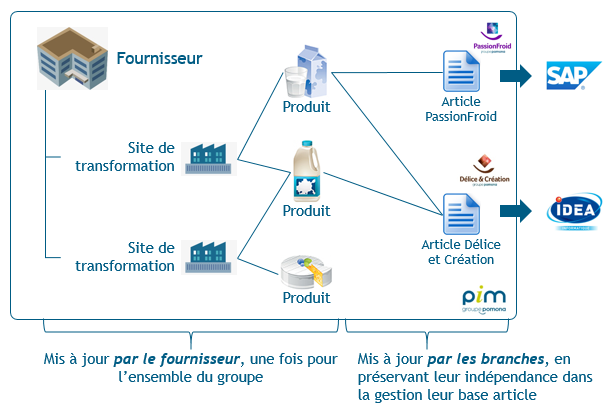
\includegraphics[width=\linewidth]{img/Produit article.png}
                \end{center}
                Dans cet exemple fictif, le type de conditionnement du lait n'a aucun impact sur les clients de la branche Délice et Création. Elle commercialise donc sous un même code article deux produits distincts.

                Pour des raisons de contrainte de conservation, la branche PassionFroid a quant à elle choisit de ne commercialiser qu'un seul produit - en brique. Elle pourrait choisir d'ouvrir un nouveau code article pour le lait en bouteille (non représenté sur le schéma ci-dessus).
                \caption{La distinction entre produit et article}
                \label{fig:produit_article}
            \end{figure}          

            \subsection{Les contrôles}

            Il a été vu que le Groupe Pomona - dans sa qualité de distributeur - n'est pas en mesure de déterminer seul les informations produit sur les marchandises qu'il commercialise.
            Néanmoins, comme cela a été vu dans la section \mref{utilisation_info_produit}, il est nécessaire que les différentes entités du Groupe soient en possession d'une information produit fiable.
            Or, avoir des données de qualité nécessite des efforts de la part des métiers, en particulier lorsque le processus n'est pas entièrement porté en interne dans la société.
            \`{A} ce titre, plusieurs étapes de contrôle ont été définies dans le processus de gestion du référentiel de données produit et article :
            \begin{description}
                \item[lorsque le fournisseur a saisi les données produit :] la personne à l'origine de la demande de référencement (en général, un acheteur) doit contrôler la cohérence des données produit
                \item[lorsque le demandeur a demandé la création d'un article :]  le gestionnaire de référentiel valide à nouveau la cohérence des informations produit
                \item[après la création article, de manière asynchrone :] le service qualité contrôle par échantillonnage les données d'une partie des produits et articles qui ont été modifiés pendant une période.
            \end{description}
            Le retour d'expérience montre que ces contrôles, loin d'être redondants, sont nécessaires pour avoir une qualité de données acceptable.
            Ces processus de contrôle sont décrits à la \reffig{fig:processus_article}.

            \begin{figure}[htpb]
                \begin{center}
                \includegraphics[width=\linewidth]{img/Processus de création article.png}
                \end{center}
                \caption{Le processus de création article}
                \label{fig:processus_article}
            \end{figure}    

            Les contrôles effectués à chacune des étapes sont les suivants : 
            \begin{description}
                \item[contrôle de la complétude des données :] vérification que les données transmises comportent l'ensemble des données attendues
                \item[contrôle de cohérence entre les données :] vérification que les informations transmises sont cohérentes entre elles (ex : un allergène présent dans la liste d'ingrédients du produit a bien été signalé comme allergène par ailleurs)
                \item[contrôle de la cohérence avec les pièces jointes :] en plus de données structurées, les fournisseurs transmettent également des fichiers portant des informations produit (ex : l'étiquette produit ou le visuel de l'emballage). Ces pièces jointes sont décrites à la section \mref{pieces_jointes}. La personne en charge du contrôle vérifie que les données transmises sont cohérentes avec ces documents.
            \end{description}

        \section{Les outils informatiques associés}
        \label{outils_infos}

        Comme vu dans la description des branches du Groupe (voir section \mref{les_branches}), les outils informatiques ne sont pas tous les mêmes sur l'ensemble des branches.
        Ainsi, les outils utilisés pour la gestion de l'information produit ne sont pas les mêmes.

            \subsection{Les branches faiblement outillées}
            
            Les branches étrangères (Pomona Suisse, Pomona Iberia), spécialistes (Délice et Création, Saveurs d'Antoine) et la branche TerreAzur sont aujourd'hui faiblement outillées.
            Cela signifie que l'information produit est en général stockée uniquement sous la forme de fichiers (essentiellement les pièces jointes, décrites à la section \mref{pieces_jointes}).
            L'ensemble des échanges avec les fournisseurs se font par mail, et les articles sont créés directement dans les systèmes de gestion par les gestionnaires de référentiel.
            Les liens entre les articles et les informations produit ne sont pas matérialisés dans les systèmes informatiques.

            \subsection{Le GIP}
            \label{GIP}

            Le GIP (Gestion de l'Information Produit) est utilisé sur la branche PassionFroid.
            C'est un système de gestion de l'information produit qui est maintenant obsolescent et en cours de remplacement.
            Il a toutefois le mérite de permettre le stockage dans une application des données et des pièces jointes relatives aux produits, avec la possibilité d'accéder aux informations produit à partir des identifiants des articles.
            C'est ce système qui a permis de pouvoir alimenter les sites de e-commerce PassionFroid et \'{E}piSaveurs avec les informations produit.
            Il est toutefois ancien, et ne propose pas de fonctionnalité d'export en masse fiable.
            Il s'agit d'une application qui n'est pas ouverte aux utilisateurs externes au Groupe, et les échanges avec les fournisseurs passent donc par des échanges de mails.

            \subsection{Le PIM}
            \label{PIM}

            Le PIM (Product Information Management) est un système de gestion de l'information produit qui a été mis en production en mai 2019, pour la branche \'{E}piSaveurs.

                \subsubsection{Description générale de l'outil}

                C'est un système qui porte l'ensemble du processus de gestion de l'information produit, tel que décrit à la \reffig{fig:processus_article}.
                Il est accessible aux fournisseurs du Groupe, qui viennent directement mettre à disposition les données et les pièces jointes.
                Cet outil porte entre autres les fonctionnalités de contrôle des informations, comme illustré à la \reffig{fig:ecran_PIM}.

                \begin{figure}[htpb]
                    \begin{center}
                    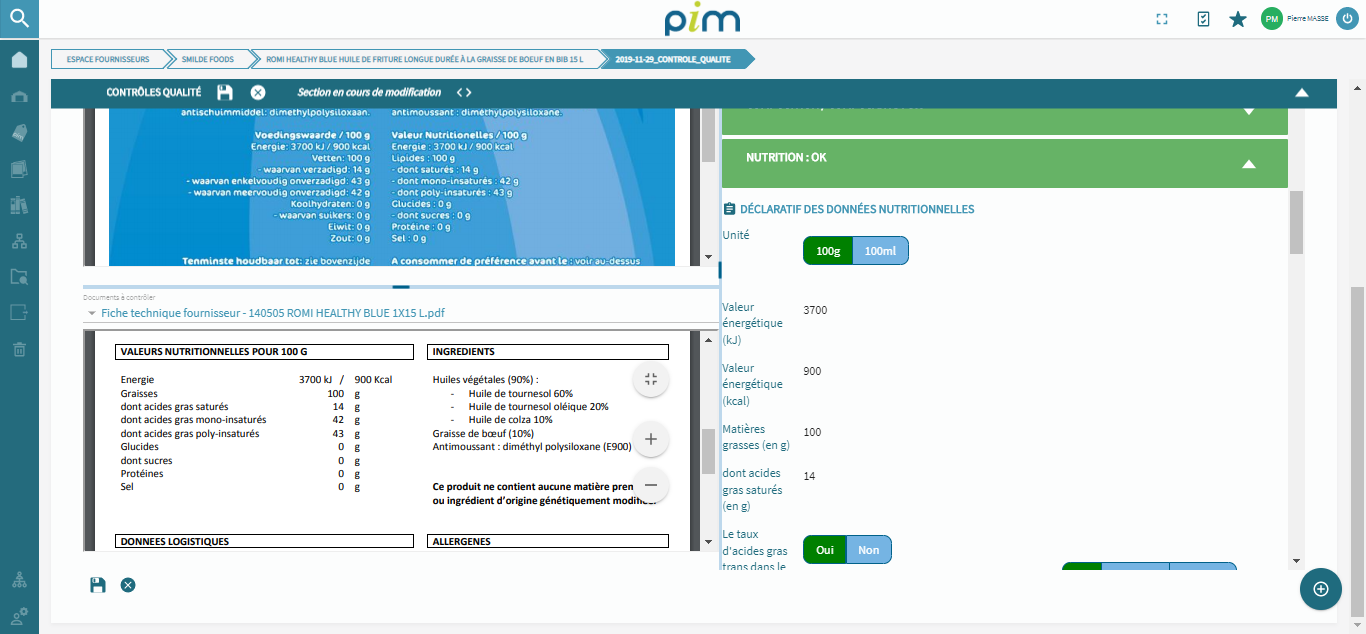
\includegraphics[width=\linewidth]{img/Ecran PIM.png}
                    \end{center}
                    Cette capture d'écran montre l'outil de contrôle des données produit. Sur la partie gauche, le contenu des pièces jointes est affiché (visuel de l'emballage en haut, fiche technique en bas), sur la droite les données qui ont été transmises par le fournisseur.
                    \caption{Une capture d'écran du PIM}
                    \label{fig:ecran_PIM}
                \end{figure} 

                \subsubsection{La GDSN}

                La GDSN (Global Data Synchronization Network) est un réseau d'échange de données produit entre industriels, distributeurs, restaurateurs, \dots
                Ce réseau est exploité par des opérateurs privés, mais le format et la chorégraphie des échanges a été standardisé par l'organisme de standardisation GS1.
                Son schéma de principe est décrit à la \reffig{fig:GDSN}.
                Sans rentrer dans le détail, au sein du Groupe Pomona l'utilisation qui en est faite est de récupérer les informations depuis ce réseau d'échange, afin de préalimenter les données produit pour les fournisseurs.
                Cette foncitonnalité permet de faire gagner du temps aux fournisseurs pour leur éviter une partie de ressaisie, mais également de limiter les erreurs.
                Toutefois, cette fonctionnalité ne permet pas à elle seule de garantir une parfaite qualité de données.
                Il s'agit uniquement d'un \og tuyau \fg, si les données en entrée ne sont pas correctes, elles ne seront pas correctes en sortie.
                Pour aller plus loin dans la compréhension de ce réseau, il est possible de consulter les ressources mises en ligne par GS1~\cite{GDSN_GS1_FR}\cite{GDSN_GS1_GLOBAL}.

                \begin{figure}[htpb]
                    \begin{center}
                    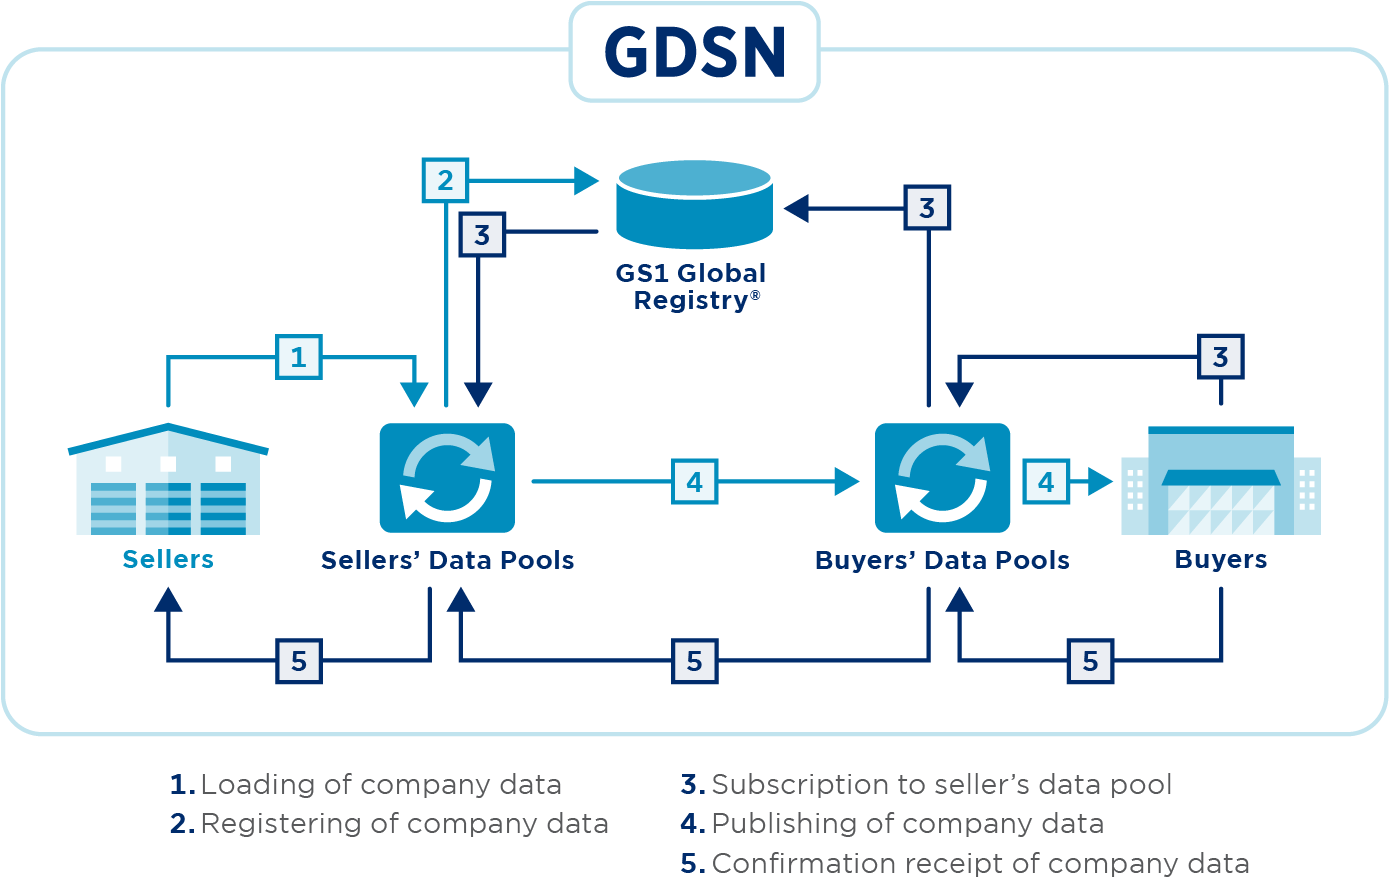
\includegraphics[width=\linewidth]{img/gdsn-schema.png}
                    \end{center}
                    \caption{Schéma de principe de la GDSN}
                    \label{fig:GDSN}
                \end{figure}                 
                
                \subsubsection{L'identification des objets dans le PIM}

                Un dernier point à connaître à propos du PIM, est la manière d'identifier l'ensemble des objets en son sein.
                Chaque objet géré (ainsi que toute version archivée) porte un identifiant unique, nommé \emph{uid} qui est totalement univoque.
                Pour la suite, on se basera sur ces uid pour faire référence à des produits stockés dans le PIM.
                Une illustration est présentée à la \reffig{fig:uid}.

                \begin{figure}[htpb]
                    \begin{center}
                    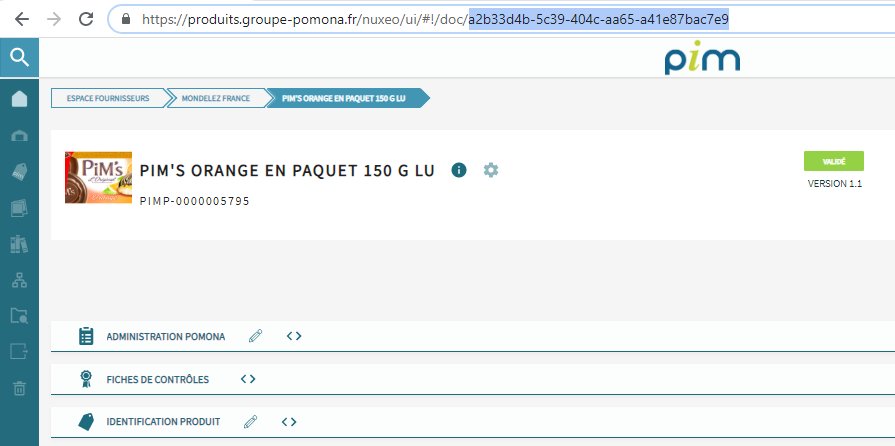
\includegraphics[width=\linewidth]{img/uid.png}
                    \end{center}
                    L'uid du produit affiché est mis en évidence dans l'url
                    \caption{L'uid d'un produit}
                    \label{fig:uid}
                \end{figure}                 

                \subsubsection{Les API}

                Un des aspects intéressants du PIM pour l'exploitation en masse des données produit, est qu'il expose des API permettant d'aller requéter l'ensemble de son contenu.
                Cela concerne à la fois les données dites structurées, mais également les pièces jointes.
                Cela rend les données produit de la branche \'{E}piSaveurs bien plus simplement accessibles que celles des autres branches.

\part{Les données}
    \chapter{Le périmètre produit}
    \label{perimetre_produit}
        \section{Accessibilité de la donnée en fonction des branches}

        Comme vu à la section \mref{outils_infos}, les systèmes d'information associés à la gestion de l'information produit offrent des niveaux d'accès hétérogènes à la donnée produit.
        Le récapitulatif par branche est le suivant : 
        \begin{description}
            \item[\'{E}piSaveurs :] on peut simplement accéder à l'ensemble des données produit, structurées, non structurées (i.e. textes longs) et pièces jointes
            \item[PassionFroid :] on a uniquement la possibilité d'exporter manuellement les données structurées articles depuis le système de gestion SAP.
            Elles permettent de produire quelques analyses quantitatives.
            Il est difficile de faire des exports en masse de l'outil de gestion de l'information produit GIP (cf. section \mref{GIP}).
            \item[TerreAzur :] idem PassionFroid, si ce n'est qu'en plus le système GIP n'est pas utilisé au sein de cette branche.
            \item[Délice et Création :] le système d'information ne permet pas d'exporter les données et donc de produire des indicateurs détaillés. On peut toutefois avoir des informations quantitatives de la part des opérationnels.
            \item[Saveurs d'Antoine :] idem Délice et Création
            \item[Pomona Suisse :] la branche est en cours de structuration, et les référentiels articles ne sont pas partagés entre les succursales. Il n'est pas possible d'obtenir d'information quantitative sur ces données.
            \item[Pomona Iberia :] idem Pomona Suisse
        \end{description}

        Pour les analyses quantitatives, on pourra se baser sur des extractions uniquement pour les branches RHD (\'{E}piSaveurs, PassionFroid, TerreAzur).
        L'ensemble des analyses portant sur les branches RHD sont produites sur la base d'extractions de leur système de gestion SAP.

        \section{Analyses quantitatives}
            \subsection{Comparatifs entre les branches}

                Les graphes de cette section ont été produits via le code présenté en annexe, au chapitre \mref{code:analyse_quantitative}.
                Les données pour les branches spécialistes (Délice et Création et Saveurs d'Antoine) sont issues d'informations fournies par le métier, hors système.


                En termes de volumétrie article (cf. \reffig{fig:volumetrie_article}, c'est TerreAzur qui possède le référentiel le plus étendu (environ 62 000 articles de marchandises actifs).
                Cela s'explique par le fait que cette branche commercialise essentiellement des produits bruts, non-préemballés (ex : des cagettes de fruits ou de légumes).
                Or, ces produits ne sont pas clairement identifiés, par exemple par un GTIN.
                Au démarrage de cette branche, afin de limiter la charge sur les gestionnaires de référentiels, le parti a été pris de créer en avance de phase l'ensemble des articles susceptibles d'être commercialisés.
                Cela s'est traduit par la création d'un grand nombre d'articles, du fait de l'application \og brutale \fg de la combinatoire des différents critères pouvant définir un produit.
                Un exemple (fictif) serait, sur les pommes : 
                \begin{itemize}
                    \item 8 variétés possibles (Gala, Golden, \dots)
                    \item 4 calibres possibles
                    \item 6 conditionnements possibles (plateau 6kg, plateau 4,5kg, \dots)
                    \item 2 catégories (I, II)
                    \item 8 origines (France, Espagne, \dots)
                \end{itemize}
                ce qui donne un total de 3072 articles uniquement sur cette gamme de produits.

                Viennent ensuite PassionFroid, et \'{E}piSaveurs, qui sont les autres \og grosses \fg branches historiques du Groupe.


                \begin{figure}[htbp]\CenterFloatBoxes
                    \begin{floatrow}
                    \ffigbox{%
                        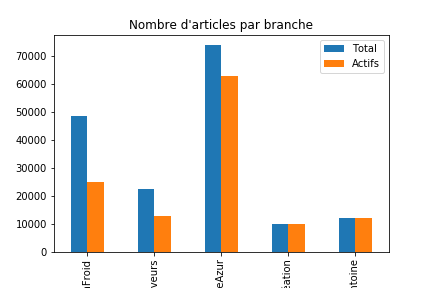
\includegraphics[width=200pt]{img/Articles par branche.png}%
                    }{%
                      \caption{Volumétrie article par branche}%
                      \label{fig:volumetrie_article}%
                    }
                    \capbtabbox[][][c]{%
                        \begin{tabular}{lccc}
\toprule
{} &  Total &  Actifs &  Marchandises \\
\textbf{Branche           } &        &         &               \\
\midrule
\textbf{PassionFroid      } &  48478 &   24898 &         24554 \\
\textbf{EpiSaveurs        } &  22498 &   12798 &         12241 \\
\textbf{TerreAzur         } &  73804 &   62789 &         62710 \\
\textbf{Délice et Création} &  10000 &       - &             - \\
\textbf{Saveurs d'Antoine } &  12000 &       - &             - \\
\bottomrule
\end{tabular}
%
                    }{%
                      \caption{Volumétrie article par branche}%
                    }
                    \end{floatrow}
                \end{figure}
                    
                Une analyse du recouvrement des référentiels montre que dans l'esemble, les branches ne travaillent pas les mêmes articles (cf. \reffig{fig:venn_article}).
                PassionFroid commercialise certains produits des branches \'{E}piSaveurs et TerreAzur, mais cela s'explique par une petite entité luxembourgeoise qui travaille des produits de tout type de stockage.
                Une réserve toutefois par rapport à cette analyse de recouvrement produit : elle sous-estime vraisemblablement lesdits recouvrements, dans la mesure où la présence de doublons n'est pas prise en compte.

                \begin{figure}[htbp]
                    \begin{center}
                    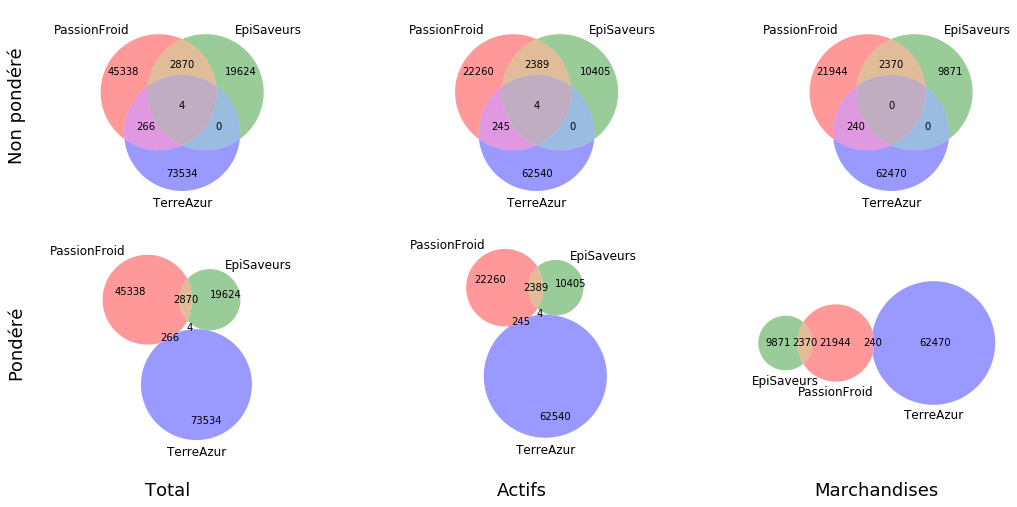
\includegraphics[width=\linewidth]{img/Diagrammes de Venn articles.png}
                    \end{center}
                    \caption{Recouvrements entre branches RHD}
                    \label{fig:venn_article}
                \end{figure}       

            \subsection{Les grands types de produits}

            Comme montré à la \reffig{fig:repart_art_categ}, on voit bien que les données ta race.

            \begin{figure}[htbp]
                \begin{center}
                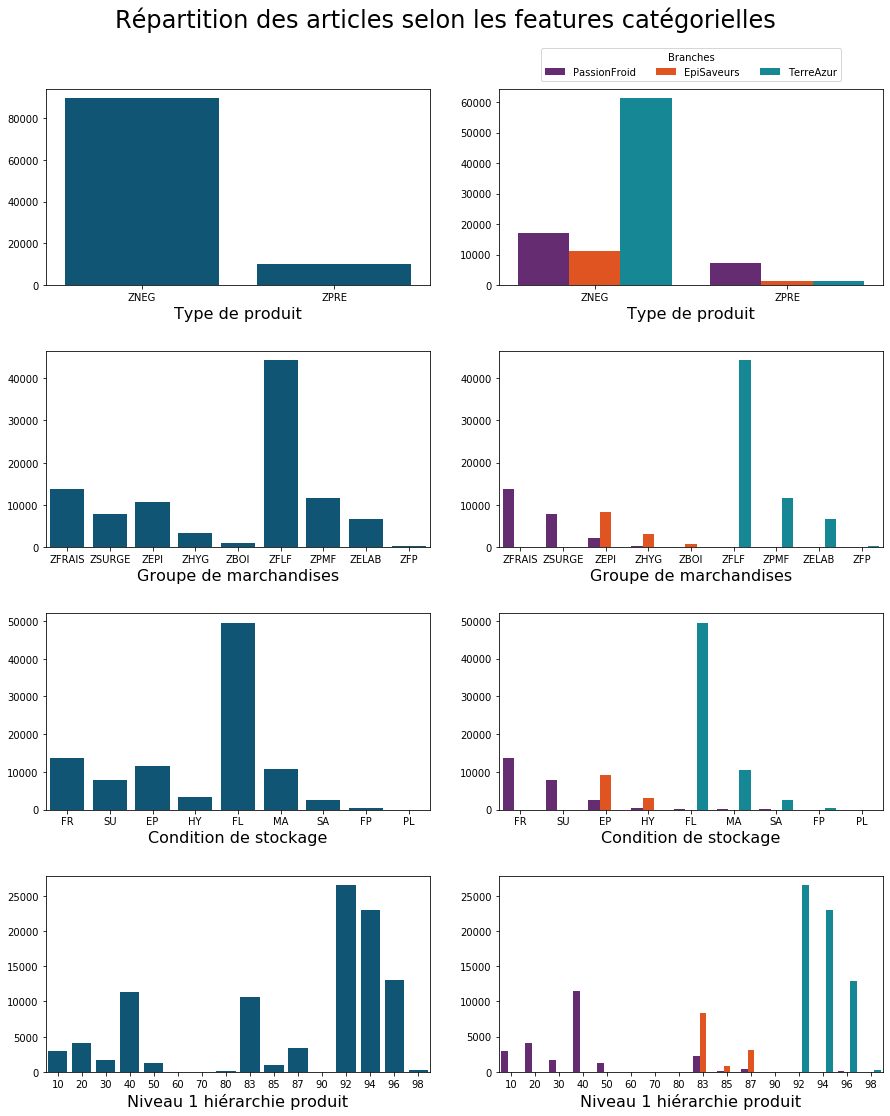
\includegraphics[width=\linewidth]{img/Repartition articles categories.png}
                \end{center}
                \caption{Répartition des articles en fonction des variable catégorielles}
                \label{fig:repart_art_categ}
            \end{figure}

            Repartition articles catégories
            Focus sur les branches Jupiter.
            Par type d'article / groupe de marchandises / groupe d'article, en retirant les articles inactifs. Toujours avec la vision article et produit (FIA).

            Ajout aussi du niveau 1 de la hiérarchie produit. Voir la possibilité de faire une représentation en 2D (type art / hiérarchie). Avec genre une heatmap qui montre que certaines de ces variables catégorielles sont en fait très très liées.

    \chapter{Les données utilisables}
        \large
        Comme vu au chapitre \mref{perimetre_produit}, les données produit ne sont simplement accessibles que pour la branche \'{E}piSaveurs.
        On se focalisera donc sur cette branche pour la suite de cette étude.
        \normalsize

        \section{Données structurées}

        Les données dites structurées sont l'ensemble des données qui peuvent prendre leurs valeurs dans un domaine restreint.
        Par exemple, ce sont les données booléennes, les choix issus de listes déroulantes, les valeurs numériques\dots
        Les principales données structurées pour les produits alimentaires dans le PIM sont : 
        \begin{description}
            \item[le code du produit :] calculé par le système
            \item[le fournisseur :] référence croisée vers le code du fournisseur
            \item[le type de produit :] épicerie, boisson alcoolisée, hygiène, chimie, boisson non-alcoolisée
            \item[le type d'unité de base :] paquet, boîte, sachet, rouleau, bouteille, pot, \dots
            \item[le GTIN du produit :] identifiant numérique unique, utilisé entre autres pour l'étiquetage sous forme de code à barres~\cite{GS1_GTIN}
            \item[les poids :] brut, net, net égoutté (pour les conserves)
            \item[le volume :] pour les produits liquides
            \item[les durées de vie :] le type (Date Limite de Consommation ou Date de Durabilité Minimale) et la durée (totale à fin de production, garantie à livraison)
            \item[les modes de conservation avant/après ouverture :] à température ambiante, au réfrigérateur puis à consommer sous 2 jours, \dots
            \item[les labels :] le(s) label(s) s'appliquant au produit (cf. section \ref{labels} page \pageref{labels})
            \item[les régimes particuliers :] Halal, Casher, Sans porc, Végétarien, Végétalien, \dots
            \item[les caractéristiques spéciales :] sans OGM, non traité par ionisation
            \item[la présence d'allergènes :] le niveau de présence de chacun des 14 allergènes réglementés (cf. section \ref{composition} page \pageref{composition})
            \item[les matières grasses utilisées :] palme, beurre, coco, tournesol, palmiste, \dots
            \item[les additifs présents :] les codes Exxx et les fonctions des additifs mis en oeuvre~\cite{additifs_regl_eu}\cite{additifs_wiki}
            \item[les données nutritionnelles obligatoires :] pour 100g ou 100mL, valeur énergétique (en kJ et kcal), matières grasses, dont acides gras saturés, Glucides, dont sucres simples, Fibres, Protéines, simplement
            \item[les données nutritionnelles facultatives :] vitamines, minéraux, omégas, \dots
            \item[les allégations nutritionnelles :] riche en, faible en, sans,\dots associé à un nutriment défini dans les 2 points précédents
            \item[le nutriscore :] note allant de A à E, définie dans la loi Santé de janvier 2016
            \item[le taux de TVA :] un des quatre taux définis dans la réglementation française
            \item[le code nomenclature douanière :] code identifiant les marchandises défini par les douanes pour la Déclaration d'\'{E}change de Biens~\cite{notions_DEB}
            \item[le pays d'origine pour la DEB :] le pays d'origine à déclarer dans la Déclaration d'\'{E}change de Biens~\cite{notions_DEB}
            \item[] 
        \end{description}
        
        
        \section{Données non structurées}
        
        Les listes d'ingrédients juste une liste ordonnées d'ingrédients triés par ordre décroissant de quantité mise en oeuvre.

        Parfois détaillé par phase, mais en général déconseillé.
        \section{Pièces jointes}
            \label{pieces_jointes}

            Dans chacune des sections, mentionner la volumétrie de données accessibles (avec les facettes migration, statuts, \& compagnie) et tout

            \subsection{Fiches techniques fournisseur}
            \subsection{\'{E}tiquettes produit}
            \subsection{Fiches logistiques fournisseur}
            \subsection{Fiches techniques et argumentaires Pomona}
        \section{Récapitulatif de la complétude des données}

        Mettre ici un ou plusieurs tableaux récapitulatifs illustrant les données possédées quantitativement.

        \section{Analyse qualitative des données}
        
        Montrer qu'un sondage basique fait que la qualité actuelle est perfectible

        Mettre également la distribution numérique des produits par fournisseur et insister sur la difficulté posée par de multiples formats

        Dire ici qu'il y a finalement beaucoup de pdf qui possèdent des textes extractibles vs. uniquement des images.

        \section{Les données \og manuellement étiquetées \fg}

        Montrer comment elles ont été produites

        Expliciter les règles de gestion qui ont été listées pendant l'étiquetage manuel

        Evaluer la cohérence entre étiquettes manuelles et contenu du PIM


\part{Les objectifs de ce projet}
    \chapter{Les cas d'usage}
        \section{Objectifs : Qualité et productivité}
        \section{La préalimentation d'information}
        \section{Le contrôle à la saisie fournisseur}
        \section{L'aide aux vérifications Pomona}
        \section{Les contrôles en masse asynchrones}
    \chapter{Les types de données à récupérer}
        \section{La composition produit}
        \section{Les données nutritionnelles}
        \section{Les données logistiques}
    \chapter{Le choix du cas d'usage}
        \section{Les multiples formats}
        \section{Les informations \og spatialisées \fg}
        \section{La complexité dans la réprésentation des données logistiques}
        \section{La moindre représentation des étiquettes}
        blablabla
        \newline
        \newline
        \emphbox{Au vu des différentes contraintes listées plus haut, on s'attachera à extraire \emph{les listes d'ingrédients} des produits \emph{alimentaires} de la branche \emph{EpiSaveurs} depuis \emph{les fiches techniques fournisseur}, en se basant sur \emph{le contenu textuel} de ces documents.}

\part{Construction du modèle}
    \chapter{Les principes généraux}
        \section{Contenu du texte d'une liste d'ingrédients}

        En général, chaque ingrédient sera présent une seule fois dans la liste.

        Le calcul d'embeddings via des modèles tels que SVD ou Word2Vec fait peu de sens.
        \newline
        \newline
        \emphbox{l'extraction des textes se fait au format \emph{Bag Of Words}, sans utiliser de notion d'IDF. L'utilsation de TF semble églament sujette à caution.}

        \section{Limitation à l'identification des listes d'ingrédients}

        On est sur une taxonomie d'informations limitée dans les fiches techniques.

        On pourrait envisager de classifier l'ensemble des textes présents dans les fiches techniques.

        Mais l'absence de données étiquetées rend cette tâche impossible. La charge d'étiquetage d'un nombre représentatif de blocs de texte de fiches techniques est trop importante pour être mise en oeuvre dans le cadre de ce projet.

        \section{Conversion de documents en texte}
        
        dire ici qu'on utilise principalement pdfminer vs. d'autres outils d'OCR.

        De plus, on partira dans un premier temps sur une transformation basique d'un document en texte, sans passer par une analyse de la localisation des textes sur le document.
            
    \chapter{Construction d'un modèle simple \og ouvert \fg}
        
    Expliciter le principe de ce modèle avec un schéma simple.

    Pas de mesure possible de la performance

        \section{Extraction des données}

        Ne garder que produits d'épicerie et boissons non alcoolisées

        \section{Conversion en blocs de texte}
        \section{Train/Test split}
        \section{Entrainement du modèle}
        \section{Calcul de la similarité}
        \section{Illustration des résultats obtenus}
    
    \chapter{Utilisation des données manuellement étiquetées}

    Expliciter pourquoi on ne peut pas faire tourner (référence parties précédentes) sur l'ensemble des données
        
        \section{Chargement des données manuellement étiquetées}

        \section{Train/Test split}

        \section{Entraînement du modèle}

        \section{Illustration des prédictions obtenues}


    \chapter{Mesure de la performance}
    
        \section{Précision}
            \subsection{Approche naïve}

            \subsection{Avec du \og text-postprocessing \fg}
        
        \section{Similarité cosinus}

        \section{Fonction de \emph{loss} spécifique}

        Expliciter les diverses distances, et pourquoi certaines sont plus pertinentes que d'autres.

        Ex : on ne garde pas la distance de Hamming
            \subsection{Distance de Levenshtein}

            \subsection{Distance de Dameray-Levenshtein}

            \subsection{Distance de Jaro}

            \subsection{Distance de Jaro-Wrinkler}
    
        \section{Cross-validation des modèles précédents}
            
            \subsection{Modèle \og ouvert \fg}

            \subsection{Modèle entraîné sur les données étiquetées manuellement}

    \chapter{Transfer learning}
        
        \section{Principe du pré-entraînement}
        
        Expliquer qu'il s'agit d'une approche hybride des 2 modèles précédents

        \section{Illustration de l'impact sur la performance}


    \chapter{Hyperparameter tuning}
            
        \section{Les paramètres ajustables}

        \section{Application d'une grid search}

\part{Travaux subséquents}
    \chapter{Opérationnalisation de cette maquette}    
        \section{Client et sponsor métier}
        \section{Définition des règles de gestion}
        \section{Mise en place d'une organisation projet}
        \section{Industrialisation du code}
        Prochaines étapes : opérationnalisation via API \\
        Documentation
        \section{Monitoring de la performance du modèle}
    \chapter{Extension des fonctionnalités offertes}
        \section{Prise en compte de nouveaux types de pièces jointes}
        \section{Utilisation d'outil d'OCR pour les pdf non structurés}
        \section{Mise en place d'outil de spatialisation des textes}
        \section{Construction d'outils d'extraction de données connexes à la composition}
        \section{\'{E}largissement aux données nutritionnelles}
        \section{Extraction d'informations complémentaires}
        \section{\'{E}valuation de la performances sur d'autres familles de produits}


\appendix
\part{Annexes}
    \chapter{Figures, tableaux et bibliographie}
        \listoftables
        \listoffigures
        \bibliographystyle{plain}
        \bibliography{./biblio} 
    \chapter{Exemple de documents fournisseur}
        \section{Fiches techniques}
        \section{\'{E}tiquettes produit}
        \section{Fiches logistiques}
    \chapter{Le code utilisé}
        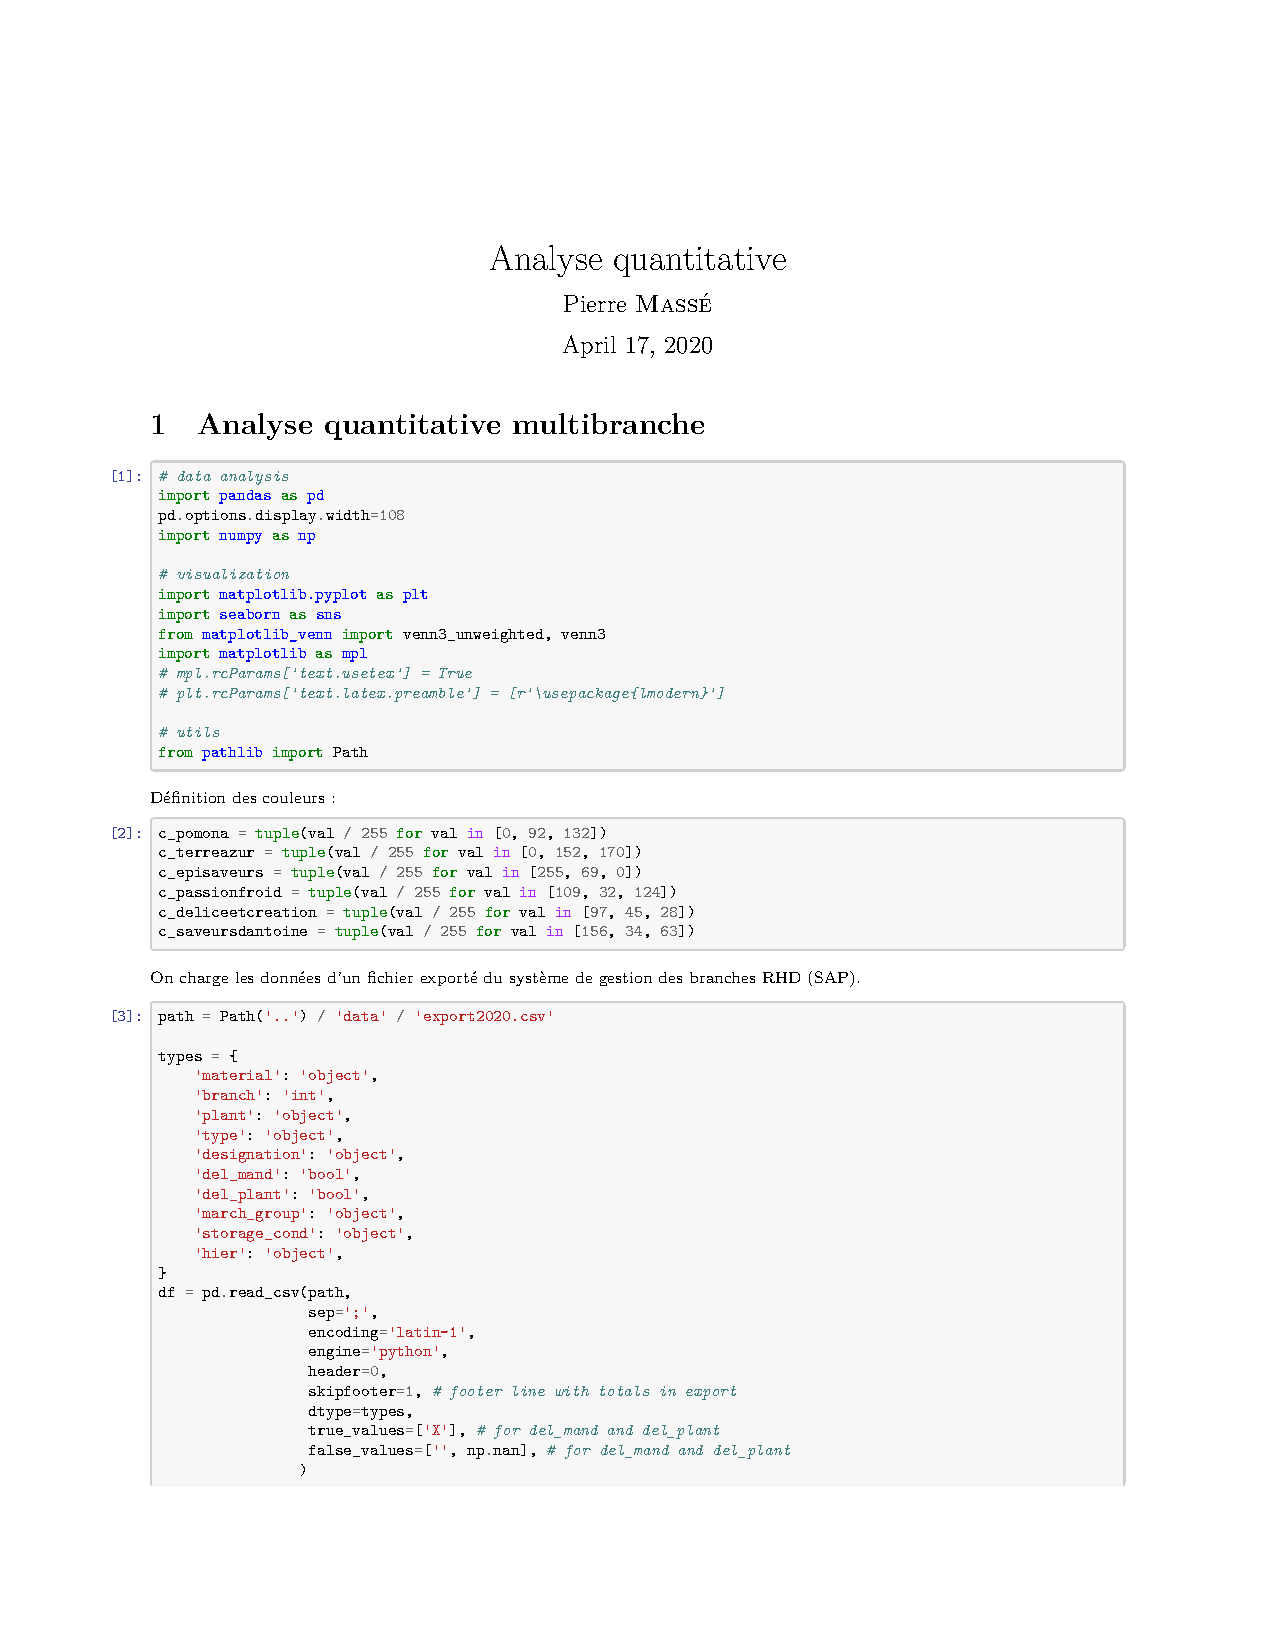
\includepdf[pages=-,
                    pagecommand={},
                    addtotoc={1,
                              section,
                              3,
                              Analyse quantitative,
                              code:analyse_quantitative}]
                    {notebooks/Analyse quantitative.pdf}

        \section{Gestion du fichier de configuration}
        Ce petit module a pour but de permettre de gérer les paramètres du progamme dans un fichier de configuration (afin de simplifier la maintenance).
        Il est utilisé dans l'ensemble des autres modules de ce projet.
        \inputminted[fontsize=\scriptsize]{python}{../src/conf.py}
        Un exemple de fichier de configuration (dont certains champs ont été anonymisés pour des raisons de confidentialité) est présenté ci-dessous.
        TODO !! Mettre le fichier ici.

        \section{Extraction des données du PIM}
            \inputminted[fontsize=\scriptsize]{python}{../src/pimapi.py}
        
        \section{Conversion des pièces jointes en textes}
            \inputminted[fontsize=\scriptsize]{python}{../src/pimpdf.py}
        
        \section{Identification des listes d'ingrédients}
            \inputminted[fontsize=\scriptsize]{python}{../src/pimest.py} 
 
\end{document}